\section{Model Formulation and Solution for Problem 1}

\subsection{Data Preprocessing}

The raw data contain 50000 jobs, 6 regions, and 3 job types, with arrivals spanning hours 0--2399. After checking field completeness and value ranges, durations are converted from minutes to hours, per-GPU power is matched by job type, and candidate regions are screened by maximum network latency. Physical quantities are neither standardized nor filtered for outliers. Forecasting data are aggregated by arrival hour, source region, and job type, including zero-demand combinations, yielding 43200 records. Hours 0--2351, 2352--2375, and 2376--2399 form the training, validation, and test sets, respectively. Scheduling uses actual test-period jobs directly; hours 2400--2405 allow unfinished execution, and hour 2406 is the terminal boundary.


\subsection{Model Formulation}

Problem 1 treats short-term GPU forecasting and baseline computing scheduling separately. Forecasts are used only for accuracy evaluation and do not enter actual scheduling.

Let $D_{rkt}$ denote newly arriving GPU demand in region $r$ for job type $k$ at time $t$,
and let $g_i$ denote the GPU demand of job $i$. Then
\begin{equation}
	D_{rkt}
	=
	\sum_{\substack{i:\,a_i=t\\
			r_i^0=r,\;k(i)=k}}
	g_i .
	\label{eq:q1_demand}
\end{equation}

This produces 18 bottom-level series, together with regional demand $D_{rt}=\sum_kD_{rkt}$, job-type demand $D_{kt}=\sum_rD_{rkt}$, and system demand $D_t=\sum_rD_{rt}$. Bottom-level series retain heterogeneity, while the three aggregate levels improve short-term forecasting stability.

Hierarchical and grouped time series require forecast reconciliation for cross-level consistency\cite{ref4}. We construct a nonnegative prior from historical demand shares and use generalized KL divergence to recover 18 cross-classified demands. This follows the reconciliation principle without directly using the Trace MinT objective.

For an aggregate demand series $y_t$,
the mean of the most recent $H$ historical hours predicts the next 24 hours:
\begin{equation}
	\hat{y}_{T+h}(H)
	=
	\frac{1}{H}
	\sum_{\tau=T-H+1}^{T}y_{\tau},
	\qquad h=1,2,\ldots,24 .
	\label{eq:q1_localmean}
\end{equation}

Here $T$ is the last observed time before forecasting. The validation set selects a window from $H\in\{24,72,168,336\}$; hours 0--2375 then forecast hours 2376--2399. Test observations do not enter model selection.

Separate regional, job-type, and system forecasts may have inconsistent totals.
We therefore use the system forecast $\hat D_t^{(S)}$ as the total-demand anchor,
proportionally rescale the regional and job-type marginals,
and obtain $\tilde D_{rt}$ and $\tilde D_{kt}$.
Let $q_{rk}$ denote the historical mean regional--job-type demand share.
A prior with the same units as GPU demand is defined as
$q^0_{rkt}=q_{rk}\hat D_t^{(S)}$;
Zero historical shares are assigned a small positive value to avoid logarithmic singularities.
Generalized KL divergence then recovers the 18 cross-classified demands:
\begin{equation}
	\begin{aligned}
		\min_{z_{rkt}\geq0}\quad
		&\sum_r\sum_k
		\left[
		z_{rkt}\ln\frac{z_{rkt}}{q^0_{rkt}}
		-z_{rkt}+q^0_{rkt}
		\right],\\
		\mathrm{s.t.}\quad
		&\sum_kz_{rkt}=\tilde D_{rt},\\
		&\sum_rz_{rkt}=\tilde D_{kt}.
	\end{aligned}
	\label{eq:q1_kl}
\end{equation}

Equation~(\ref{eq:q1_kl}) keeps the two sets of marginals fixed while retaining the historical structure of the 18 demands. WAPE, RMSE, and MAE evaluate forecasts against demand at the same hour 24 hours earlier.

Baseline computing scheduling uses actual jobs arriving during hours 2376--2399.
Let job $i$ have duration $d_i$ and source region $r_i^0$.
Network latency determines candidate regions $R_i$.
Real-time inference jobs start immediately on arrival;
batch inference and AI training jobs have candidate start times $S_i$ consistent with earliest start, latest completion, and the terminal boundary at 2406.
The binary variable $x_{irs}$ indicates whether job $i$ starts in region $r$ at time $s$.

Job durations retain minute precision, while resource capacities are evaluated hourly.
The actual occupancy of interval $[t,t+1)$ for job $i$ starting at $s$ is
\begin{equation}
	\rho_{ist}
	=
	\max\left\{
	0,\,
	\min(s+d_i,t+1)-\max(s,t)
	\right\}.
	\label{eq:q1_overlap}
\end{equation}

Equation~(\ref{eq:q1_overlap}) gives hourly GPU and power occupancy.
The AI IT power of job $i$ during full execution is
$p_i=g_iP^{GPU}_{k(i)}$.
The effective IT power available to AI jobs in region $r$ at time $t$ is
\[
A_{rt}
=
\max\left\{
0,\,
\min\left(
P^{IT,\max}_r-P^{NonAI}_{rt},
\frac{P^{Facility,\max}_r}{PUE_r}-P^{NonAI}_{rt}
\right)
\right\}.
\]
The main resource constraints are
\begin{equation}
	\begin{aligned}
		&\sum_{r\in R_i}\sum_{s\in S_i}x_{irs}=1,
		&&\forall i,\\
		&\sum_i\sum_{s\in S_i}
		g_i\rho_{ist}x_{irs}
		\leq G^{ava}_{rt},
		&&\forall r,t,\\
		&\sum_i\sum_{s\in S_i}
		p_i\rho_{ist}x_{irs}
		\leq A_{rt},
		&&\forall r,t .
	\end{aligned}
	\label{eq:q1_capacity}
\end{equation}

Equation~(\ref{eq:q1_capacity}) ensures unique execution and feasible GPU and power occupancy. Candidate sets $R_i$ and $S_i$ exclude combinations violating latency, time windows, or the terminal boundary.

Problem 1 excludes prices, emissions, renewables, and storage,
providing a neutral computing baseline for subsequent computing--electricity coordination.
First minimize cross-region migrated GPU work,
then minimize cumulative waiting of flexible jobs conditional on the optimal first-level objective:
\begin{equation}
	\begin{aligned}
		\min\quad
		F_1
		&=
		\sum_i
		\sum_{\substack{r\in R_i\\r\neq r_i^0}}
		\sum_{s\in S_i}
		g_id_ix_{irs},\\
        \text{subject to }F_1=F_1^{*}\text{,}\qquad
		\min\quad
		F_2
		&=
		\sum_{i\in I^{\mathrm{flex}}}
		\sum_{r\in R_i}\sum_{s\in S_i}
		(s-e_i)x_{irs}.
	\end{aligned}
	\label{eq:q1_objective}
\end{equation}

Here $F_1$ measures migrated GPU work and $F_2$ measures cumulative waiting of flexible jobs.


\subsection{Results and Model Validation}

The validation set gives the lowest overall WAPE at $H=72$. Historical data from hours 0--2375 therefore forecast the 18 GPU-demand series for hours 2376--2399.

The cumulative AI-training GPU demands in RegionD, RegionE, and RegionF are
407683, 292000, and 296143, respectively,
substantially above the corresponding values in RegionA, RegionB, and RegionC:
63070, 62551, and 58899.
Bottom-level hourly demand also contains many low values and random spikes,
making direct forecasts of the 18 fine-grained series sensitive to random job arrivals.

\begin{table}[H]
	\centering
    \caption{Forecast errors of the hierarchical model and the 24-hour same-hour baseline}
	\label{tab:q1_forecast}
	
	\fontsize{10.5pt}{12pt}\selectfont
	\renewcommand{\arraystretch}{0.88}
	
	\begin{tabular}{ccccccc}
		\toprule
        \multirow{2}{*}{\textbf{Period}}
        & \multicolumn{3}{c}{\textbf{Hierarchical local mean}}
        & \multicolumn{3}{c}{\textbf{24-hour same-hour baseline}}\\
		\cmidrule(lr){2-4}\cmidrule(lr){5-7}
		& \textbf{WAPE} & \textbf{RMSE} & \textbf{MAE}
		& \textbf{WAPE} & \textbf{RMSE} & \textbf{MAE}\\
		\midrule
        Validation
		& 0.7241 & 45.7417 & 23.6915
		& 1.0957 & 69.9249 & 35.8495\\
		
        Test
		& 0.6519 & 53.4704 & 26.3323
		& 0.8740 & 72.8628 & 35.3032\\
		\bottomrule
	\end{tabular}
\end{table}


Table~\ref{tab:q1_forecast} shows that all three errors of the hierarchical model are below the baseline in both validation and test periods. The problem separately requires short-term forecasting and final-period computing scheduling; forecasts assess demand predictability, while actual jobs arriving during hours 2376--2399 remain the scheduling input so that forecasting errors cannot alter job-level feasibility. Validation and test WAPE of 0.7241 and 0.6519 show that sparse demand and random spikes remain difficult to predict. Lower test WAPE and higher RMSE are consistent: WAPE is normalized by total observed demand, whereas RMSE is more sensitive to a few large errors.

\begin{figure}[H]
	\centering
	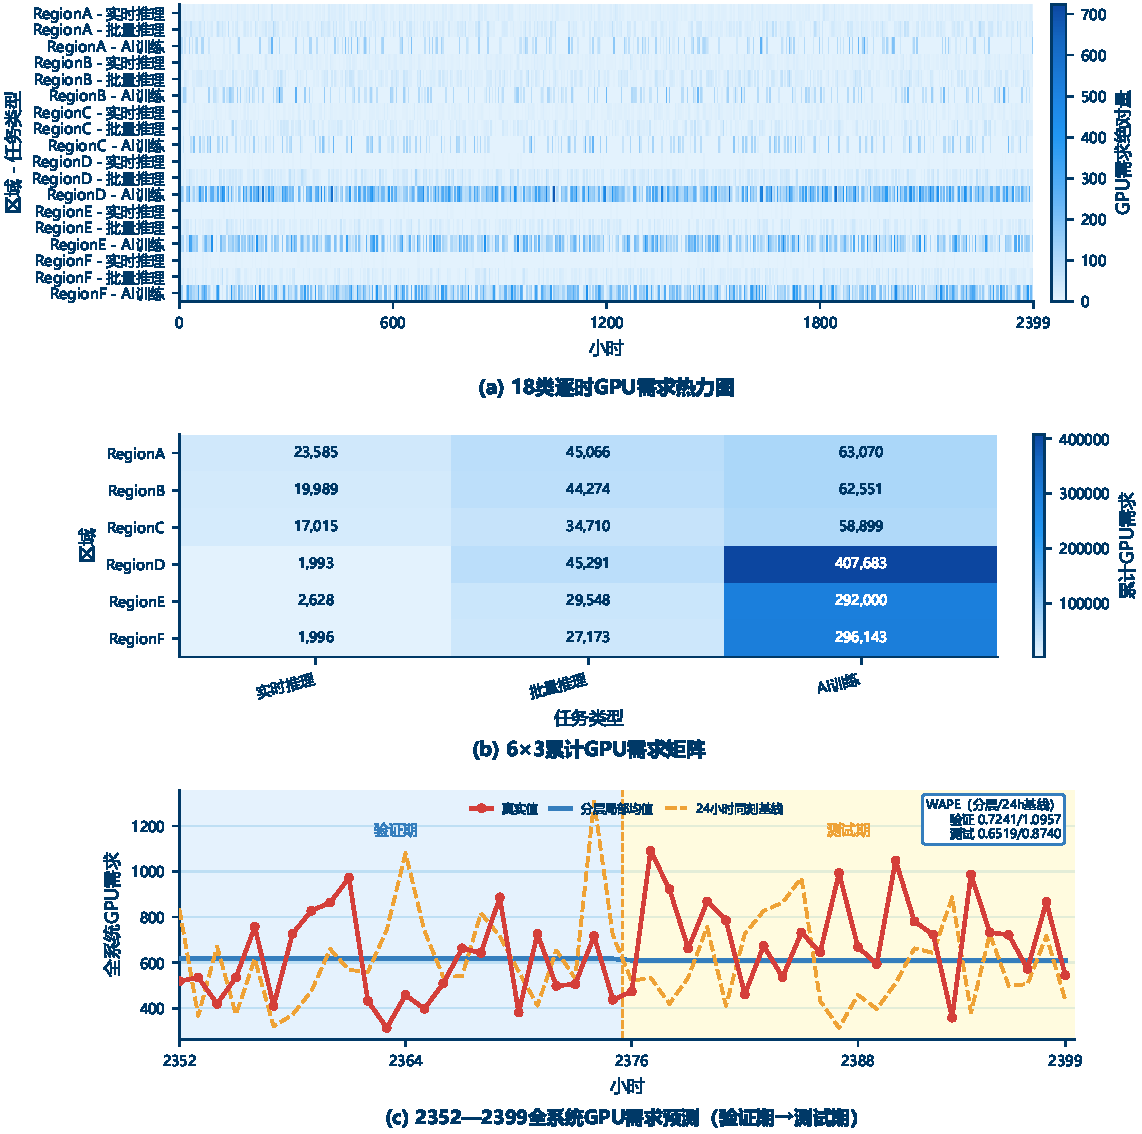
\includegraphics[width=0.80\textwidth]{figures/q1_group1_demand_structure.pdf}
    \caption{GPU-demand heterogeneity and hierarchical short-term forecasts}
	\label{fig:q1_forecast}
\end{figure}

Figure~\ref{fig:q1_forecast} shows that the model captures short-term demand levels rather than random single-hour spikes.

The 538 actual jobs arriving during hours 2376--2399 undergo two-level optimization using Equation~(\ref{eq:q1_objective}).

\begin{table}[H]
	\centering
    \caption{Baseline computing scheduling results}
	\label{tab:q1_dispatch}
	
	\fontsize{10.5pt}{12pt}\selectfont
	\renewcommand{\arraystretch}{0.88}
	
	\begin{tabular}{cc}
		\toprule
        \textbf{Metric} & \textbf{Result}\\
		\midrule
        Number of jobs & 538\\
        First-level objective $F_1^*$ & $0$ GPU$\cdot$h\\
        Local execution rate & 100\%\\
        Second-level objective $F_2^*$ & 3 h\\
        Relative optimality gap & 0\\
		\bottomrule
	\end{tabular}
\end{table}


In Table~\ref{tab:q1_dispatch}, $F_1^*=0$ and $F_2^*=3$ h. All 538 jobs finish in their source regions; the current resources permit feasible execution without migration.

\begin{figure}[H]
	\centering
	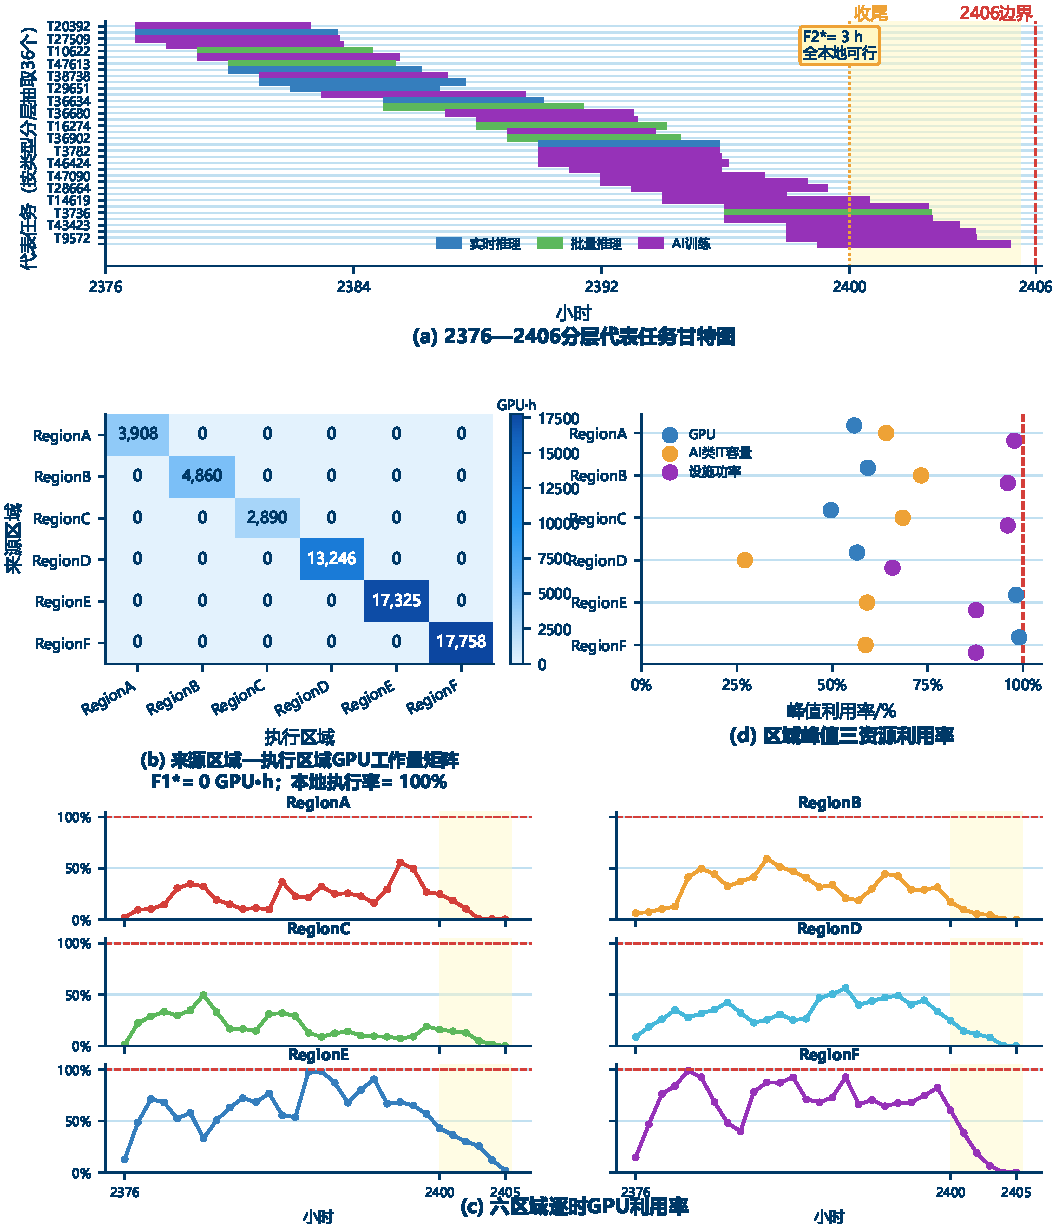
\includegraphics[width=0.75\textwidth]{figures/q1_group2_core_results.pdf}
    \caption{Baseline computing schedule and multiple-resource occupancy}
	\label{fig:q1_dispatch}
\end{figure}

Figure~\ref{fig:q1_dispatch} shows completion of all final-period jobs before 2406 and a regional GPU-work matrix with nonzero entries only on its main diagonal. RegionE and RegionF approach GPU limits during some hours, while certain eastern regions are constrained by facility power.

The hierarchical model has lower WAPE than the 24-hour same-hour baseline in all 84 rolling out-of-sample windows; a one-sided Wilcoxon test gives $p=8.55\times10^{-16}$.

The median WAPE difference between reconciled and direct forecasts is $-3.05\times10^{-4}$ ($p=0.216$). Maximum regional and job-type marginal closure errors are both $6.82\times10^{-13}$, and the 18-class aggregate error is $4.11\times10^{-10}$. Reconciliation ensures cross-level closure rather than improving accuracy.

\begin{figure}[H]
	\centering
	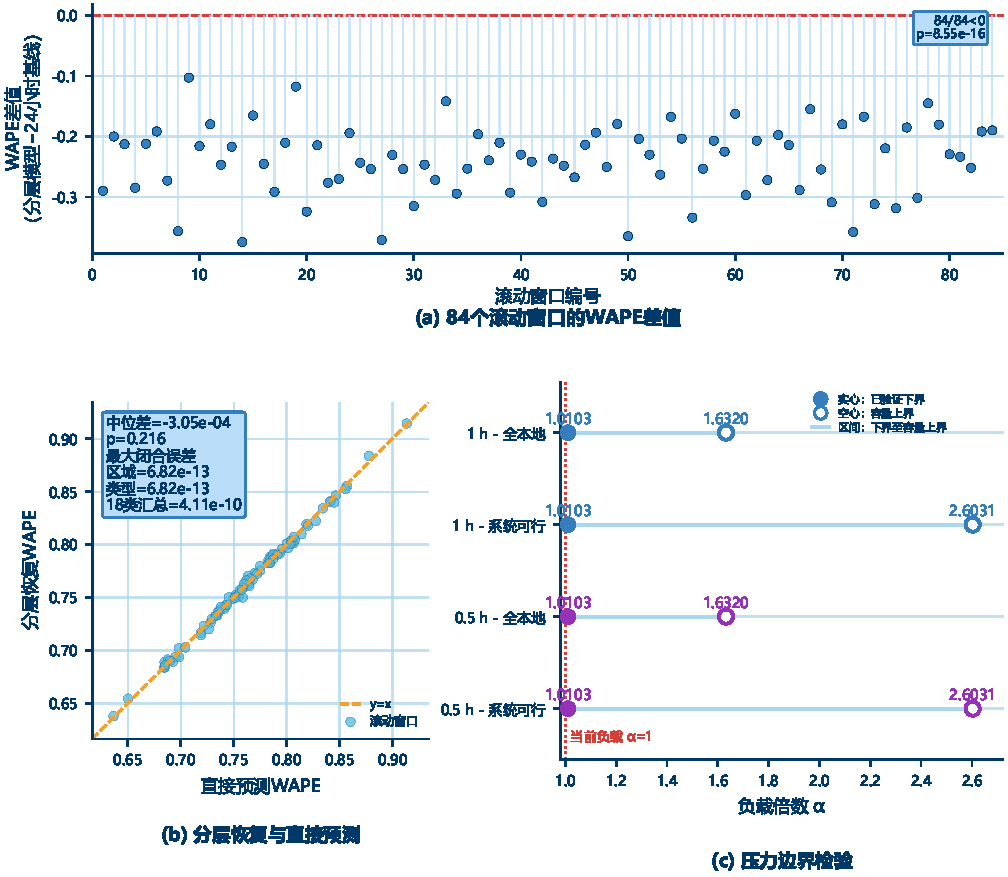
\includegraphics[width=0.80\textwidth]{figures/q1_group3_validation_robustness.pdf}
    \caption{Forecast stability and computing-schedule stress boundaries}
	\label{fig:q1_validation}
\end{figure}

In Figure~\ref{fig:q1_validation}, the verified feasible lower bound on load multiplier $\alpha$ is 1.0103. The theoretical capacity upper bounds for fully local execution and cross-region coordination are 1.6320 and 2.6031; these latter values are not verified exact critical thresholds.

Recomputation with 0.5-hour granularity still yields $F_1^*=0$, while cumulative waiting falls from 3 h to 2 h. The conclusion that migration is unnecessary remains unchanged. Unique execution, immediate real-time starts, latency, deadlines, and all capacity constraints show no violations.

Problem 1 thus establishes short-term demand forecasts and a computing-only baseline for comparison after Problem 2 introduces energy factors.
